\documentclass[t]{beamer}
\usetheme{Boadilla} %\usetheme{Goettingen}
\usefonttheme{serif}
\usefonttheme{professionalfonts}
\usecolortheme{beaver}
\setbeamertemplate{itemize item}{•}
\setbeamertemplate{itemize subitem}{◦}
\setbeamertemplate{itemize subsubitem}{—}
\setbeamertemplate{section in toc}[default] % include section on outline slide
\setbeamertemplate{subsection in toc}[default] % include subsection on outline slide
\beamertemplatenavigationsymbolsempty % no bullets on outline slide
\setbeamercovered{transparent=30} % global setting for slide builds (enabled by the <1-2> codes after \item)

\usepackage{fontspec, setspace, tabu, booktabs, multirow, url, amsmath, colortbl}
%\usepackage[shortcuts]{extdash}
\usepackage[sort&compress,super]{natbib}

% Use these with \footnotemark, \footnotetext & \bibentry if you want references to show up on each slide
%\usepackage{bibentry} 
%\nobibliography*

% misc hacks
\def\newblock{\hskip .11em plus .33em minus .07em}
\definecolor{lgray}{gray}{0.7}
\newenvironment{hl}{\usebeamercolor[fg]{frametitle}}

% fonts
\setmainfont[Numbers={Lining}]{Linux Libertine O} \setsansfont{Linux Biolinum O} \setmonofont{Linux Libertine Mono O}
%\newfontfamily{\charis}{Charis SIL}
%\newenvironment{ipa}{\large\charis}{}%
\renewcommand\url{\begingroup \def\UrlLeft{}\def\UrlRight{}\urlstyle{same}\Url} % set URLs in same font as surrounding text

% replacement for itemize environment
\newenvironment{itm}{%
	\setlength{\leftmargini}{0.5em}%
	\setlength{\leftmarginii}{1em}%
	\begin{itemize}}{\end{itemize}%
}

% misc abbreviations
\newcommand{\term}[1]{“#1”} % first occurrence of technical terms
\newcommand{\ac}[1]{\textsc{#1}} % acronyms % \newcommand{\ac}[1]{\MakeUppercase{#1}}
\newcommand{\lat}[1]{\textit{#1}} % foreign words and abbreviations
\newcommand{\psola}{\ac{psola}™}
\newcommand{\fo}{ƒ₀} % font problems? might work as {\(f_0\)}
\newcommand{\eg}{\lat{e.g.}}
\newcommand{\ie}{\lat{i.e.}}
\newcommand{\etseq}{\lat{et seq}}
\newcommand{\etc}{\lat{etc}}
\newcommand{\intal}{\lat{inter alia}}
\newcommand{\ph}{\lat{post hoc}}
\newcommand{\Ph}{\lat{Post hoc}}
\newcommand{\aka}{\textsc{aka}}
\newcommand{\vs}{\lat{vs.}}
\newcommand{\vv}{\lat{vice versa}}
\newcommand{\perse}{\lat{per se}}
\newcommand{\slsh}{/‌} % contains a zero-width non-joiner after the slash, to allow line breaking

% Automatically insert overview/roadmap slide at start of each section
\AtBeginSection[]{%
\begin{frame}<beamer>
    \frametitle{Overview}
    \tableofcontents[currentsection]
  \end{frame}
}

\title[Prosody, intelligibility \& familiarity]{Prosody, intelligibility and familiarity\\in speech perception}
%\subtitle[short subtitle]{long subtitle}
\author[McCloy]{Daniel~McCloy} 
\institute[UW]{Department of Linguistics, University of Washington}
\date[2013.05.31]{2013 May 31}
\subject{Linguistics, Phonetics, Speech Perception}

\begin{document}

%===== TITLEPAGE =====%
\frame{\titlepage}


%===== TABLE OF CONTENTS =====%
\begin{frame}{Overview}
	\tableofcontents{}
\end{frame}

%===== MOTIVATION =====%
\section{Motivation}

\subsection{Why study intelligibility?}
\begin{frame}{Why study intelligibility?}
	\begin{itm}
		\item<1-3> \emph{What is the same across talkers?}
		\begin{itm}
			\item Can tell us about the brain’s speech processing system
			\begin{itm}
				\item One example: target–masker similarity
			\end{itm}
		\end{itm}
		\item[]
		\item<2-3> \emph{What is different across talkers?}
		\begin{itm}
			\item Applications to assistive hearing device design (acoustics, signal processing)
			\item Applications to speech therapy, pedagogy (articulation)
		\end{itm}
		\item[]
		\item<3> \emph{What is different across groups?}
			\begin{itm}
				\item Cross-linguistic differences in speech perception
				\begin{itm}
					\item Insight into “active” phonological features
				\end{itm}
			\end{itm}
	\end{itm}
\end{frame}

\subsection{Why study prosody?}
\begin{frame}{Why study prosody?}
	\begin{itm}
		\item<1-3> Hearing aids: prosodic changes easier than segmental changes
		\item[]
		\item<2-3> Natural distinction: segmental \vs\ supersegmental
		\begin{itm}
			\item Duration, \fo, and intensity not phonemic in English as spoken here\\(secondary cues)
		\end{itm}
		\item[]
		\item<3> Bottom-up approach using acoustic predictors: conflicting results
	\end{itm}
\end{frame}

%===== BACKGROUND =====%
\section{Background}

\begin{frame}{What impacts intelligibility?}
	\begin{columns}
		\begin{column}{0.5\textwidth}
		\begin{itm}
			\item<1-2> Language user properties
			\begin{itm}
				\item Speech style
				\item Listener experience with language/dialect
				\item Intrinsic individual differences?
				\item Gender?
			\end{itm}
		\end{itm}
		\end{column}
		\begin{column}{0.5\textwidth}
		\begin{itm}
			\item<2> Signal properties
			\begin{itm}
				\item Speech rate
				\item Vowel space size
				\item Pitch range
			\end{itm}
		\end{itm}
		\end{column}
	\end{columns}
	
\end{frame}

%===== METHODS =====%
\section{Methodology}

\begin{frame}{General approach}
	\begin{itm}
		\item<1-3> Top-down \vs\ bottom-up
		\begin{itm}
			\item<2-3> Not a perfect split:
			\begin{itm}
				\item Vowel reduction (formant values) affected by phrasal accent
				\item Consonant reduction (spirantization, glottalization, flapping) affected by prosody
				\item Duration is secondary cue to phonemic distinctions
				\item Pitch is (subtly) affected by vocal tract constrictions (\ie, consonants)
			\end{itm}
		\end{itm}
		\item[]
		\item<3> Why use resynthesis?
		\begin{itm}
			\item Advantage: Less work than parametric synthesis; natural-sounding voices
			\item Disadvantage: risk of distortion; real voices!
		\end{itm}
	\end{itm}
\end{frame}

\begin{frame}{Stimulus design}
	\begin{itm}
		\item Careful recordings of parallel sentences (head mounted mics, low noise floor, coached to standardize prosody)
		\item[]
		\item Five \ac{pnw} male talkers included in corpus; three selected for resynthesis
		\item[]
		\item Duration, intensity \& pitch swapped between all possible pairs of talkers
	\end{itm}
\end{frame}

\begin{frame}{Resynthesis (1 of 3)}
	\begin{itm}
		\item Hand-correction of pitch epoch marks (“pulses”) to ensure consistent phase with respect to waveform\\
			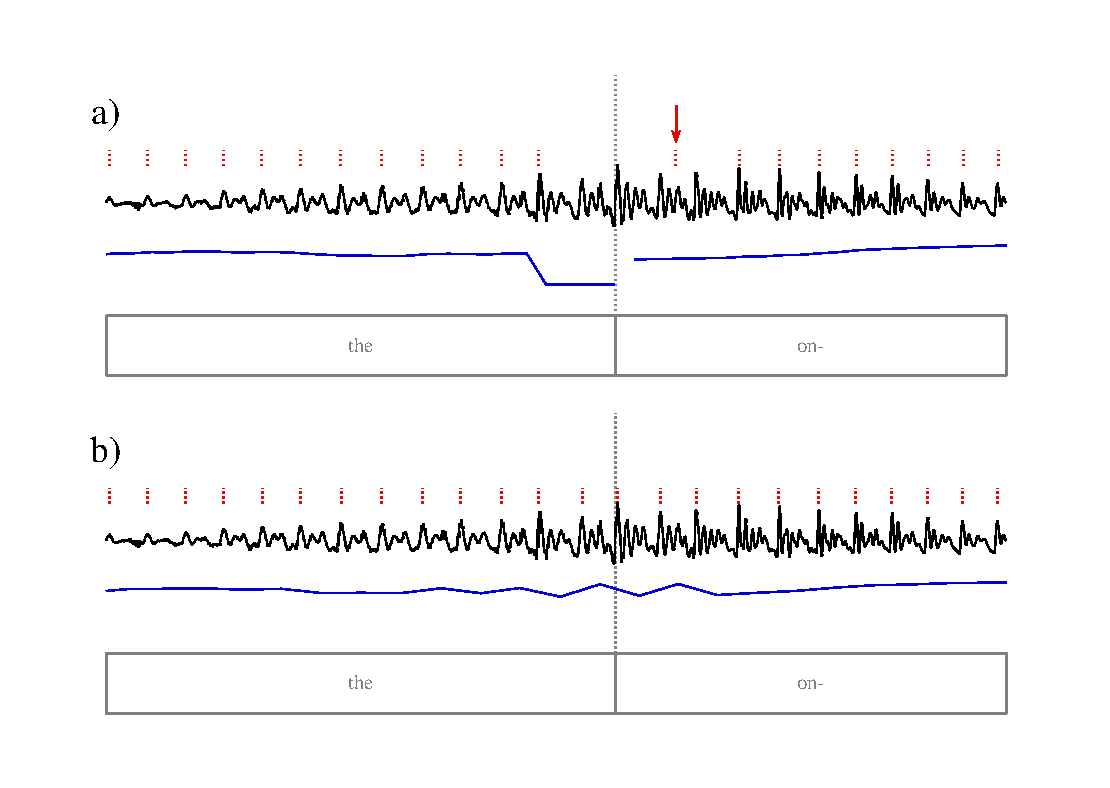
\includegraphics[width=\textwidth,height=0.7\textheight,keepaspectratio]{../figures/creakJitterShimmer/creakJitterShimmer.eps}
%			\caption[Handling of creaky voicing in resynthesis]{Illustration of method for handling creaky\-/voiced portions of speech.  (a)~Excerpt of Talker~\ac{b}’s recording of sentence 33–05, in which vowel hiatus is resolved with light creaky voicing.  The waveform (black) is overlaid with Praat’s auto\-/detected pulse marks (dotted red lines) and pitch track (dashed blue line).  Note the missed cycles on either side of the red arrow, and the phase\-/shift of all pulses right of the arrow.  (b)~The same span of speech after manual correction of pulses, and a (jittery, but continuous) pitch track generated from the corrected pulses.\label{fig:JitShim}}
	\end{itm}
\end{frame}

\begin{frame}{Resynthesis (2 of 3)}
	\begin{itm}
		\item Dynamic time warping of pitch and intensity 
		\item[] 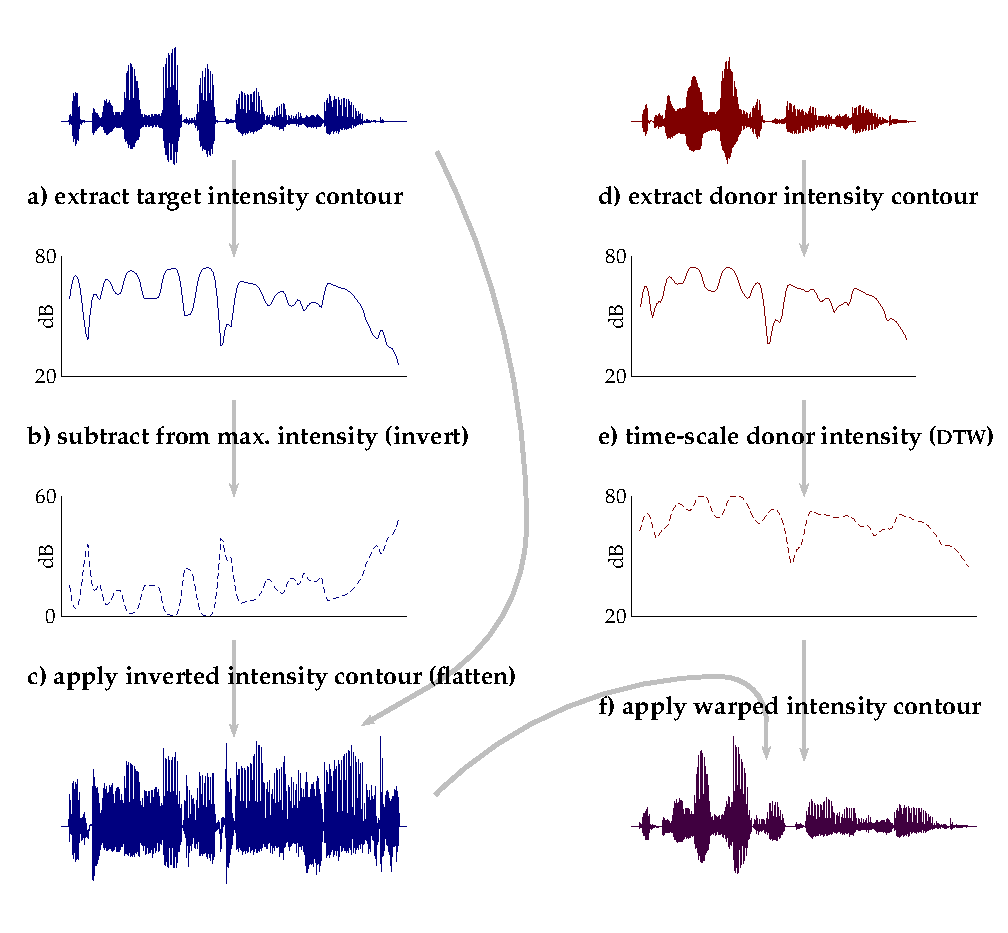
\includegraphics[width=\textwidth,height=0.75\textheight,keepaspectratio]{../figures/intensity/intensity2.eps}
%				\caption[Intensity scaling in resynthesis]{Illustration of the method used to scale intensity.  (a)~Intensity contour is extracted from target waveform (blue).  (b)~The intensity contour of the target signal is inverted, by subtracting each intensity point from the maximum intensity.  (c)~Target intensity is \term{neutralized} or \term{flattened} by multiplying the target signal by the inverted intensity contour.  (d)~Intensity contour is extracted from the prosodic donor signal (red).  (e)~The prosodic donor intensity contour is time\-/scaled syllable\-/by\-/syllable via dynamic time warping (\ac{dtw}) to match the temporal pattern of the target signal.  (f)~The intensity\-/neutralized target signal is multiplied by the time\-/warped donor intensity contour (purple).  The signal is now ready for \psola{} resynthesis of duration and pitch.\label{fig:IntenManip}}
	\end{itm}
\end{frame}

\begin{frame}{Resynthesis (3 of 3)}
	\begin{itm}
		\item \psola{} algorithm as implemented in Praat
		\item[]
		\item (Show demo)
%		\item Graphic of how it works?  Demo?
	\end{itm}
\end{frame}

%===== RESULTS =====%
\section{Results}

%===== DISCUSSION =====%
\section{Discussion}

%===== REFERENCES =====%
% Don't give this its own section, unless you want an auto-generated return to the outline slide just before it
%\begin{frame}{References}
%	\tiny
%	\bibliography{bibFileName}
%	\bibliographystyle{apa-good}		
%\end{frame}


\subsection{Acknowledgments} % include if you want on the outline / in PDF bookmarks
\begin{frame}{Acknowledgments}
	\begin{itm}
		\centering
		\item[] Thanks to:
		\item[] 
		\item[] Richard~Wright, Sharon~Hargus, Erick~Gallun, Gina-Anne~Levow, Pam~Souza
		\item[] 
		\item[] Jennifer~Haywood, Gus~McGrath, Steve~Moran, Darren~Tanner, members~of~the~UW~Phonetics~Lab
		\item[] 
		\item[] Sherry~Brown, David~Adams, Dennis~Lamb, Bill~Moody, Larry~BonJour, Bill~Talbott, David~Knechteges, Bi~Nyan-Ping, Zev~Handel, Chris~Stecker, KC~Lee
		\item[] 
		\item[] Sarala~Puthuval
	\end{itm}
\end{frame}

\end{document}

%\begin{frame}{TableExample}
%	\begin{itm}
%		\item<1-2> foo
%		\item[] % Typically you'll want a blank line before and after the table item
%		\item[]<2> % [] suppresses bullet for table item
%		{\small
%		\begin{tabu} to 0.9\textwidth {l l X}
%			\toprule
%			\arrayrulecolor{lgray}
%			foo & foo & foo\\ \midrule
%			foo & foo & foo\\ \midrule
%			foo & foo & foo\\
%			\arrayrulecolor{black}\bottomrule
%		\end{tabu}
%		}%small
%		\item[] % Typically you'll want a blank line before and after the table item
%		\item<3> foo takeaway
%	\end{itm}
%\end{frame}

